\chapter{Algoritmo de clasificación}
\label{chap:algoritmo}

 \graphicspath{{Chapter5/Figuras/}{Chapter6/Figs/PDF/}{Chapter4/Figs/}}

En este capítulo se describirá el proceso de desarrollo del algoritmo de clasificación. Este proceso se puede apreciar en la Fig.~\ref{fig:Flujo_desarrollo}.

\begin{figure}[hbt!]
\centering
\includegraphics[width=0.25\textwidth]{Flujo_desarrollo.pdf}
\caption{Diagrama de flujo del desarrollo del algoritmo de clasificación.}
\label{fig:Flujo_desarrollo}
\end{figure}

En la Fig.~\ref{fig:datos_ejemplo} se definen algunos conceptos que se usarán a lo largo de este capítulo. Estos conceptos describen el contenido de un dataset. Cada dataset esta compuesto por \textit{instancias}. Cada instancia tiene un conjunto de \textit{características} y es asignada a una \textit{clase}.

\begin{figure}[hbt!]
\centering
\includegraphics[width=\textwidth]{datos_ejemplo.pdf}
\caption{Partes de un dataset.}
\label{fig:datos_ejemplo}
\end{figure}


\subsection{Recolección de datos}
Como se expresó en el concepto óptimo de solución, se usará en esta tesis un algoritmo supervisado para realizar la clasificación del estilo de manejo. Esto significa que los datos usados para entrenar y validar el algoritmo necesitan estar previamente clasificados.

Debido a la poca disponibilidad de esta clase de datos (datos de manejo clasificados como agresivos o no) se decidió utilizar un dataset disponible en Kaggle, el cuál tenía como objetivo desarrollar una estrategia inteligente para la caja de cambios. Este dataset fue generado usando el puerto OBD2 de un vehículo y un IMU para obtener data durante varios recorridos. Sin embargo, no solo se registró datos de los sensores, sino que también se registro datos categóricos de acuerdo al viaje realizado. En la Tabla~\ref{diag:Dataset} podemos observar todos los datos que contiene este dataset.

\bgroup
\def\arraystretch{1.5}%  1 is the default, change whatever you need
\begin{table}[bth!]
\centering
\caption[Características o features del dataset]{Características o features del dataset.}
\begin{tabular}{@{}ll@{}}
\toprule
Datos de sensores (series temporales) & Datos Categóricos \\ \midrule
Tiempo (segundos) & Número de pasajeros (0 - 5) \\
Velocidad del vehículo (\SI{}{m/s}) & Carga del auto (0 - 10) \\
Número de cambio & Aire acondicionado (0 - 10) \\
Carga del motor (\%) & Apertura de ventanas (0 - 10) \\
Aceleración total (\SI{}{m/s^2}) & Volumen del radio (0 - 10) \\
RPM del motor & Intensidad de lluvia (0 - 10) \\
Pitch  & Visibilidad (0 - 10) \\
Aceleración Lateral (\SI{}{m/s^2}) & Bienestar del conductor (0 - 10) \\
 & Prisa del conductor (0 - 5) \\ \bottomrule
\end{tabular}
\label{diag:Dataset}
\end{table}
\egroup



Como se puede apreciar en la Fig.~\ref{fig:duracion_datps}, estos datos consisten en 39 viajes grabados, los cuales hacen en total \SI{21.5}{h} de manejo grabadas a una frecuencia de \SI{100}{Hz}. Estos datos se usarán para diseñar y probar el algoritmo de clasificación.

\begin{figure}[hbtp!]
\centering
\includegraphics[width=\textwidth]{duracion_viajes.pdf}
\caption{Duración de cada viaje grabado en el dataset.}
\label{fig:duracion_datps}
\end{figure}

Como se observa en la Tabla ~\ref{diag:Dataset}, ninguna de estas características es la clase "agresividad al conducir" o "estilo de conducción". Por lo que se tendrá que definir a que clase pertenecen estos datos. Para esto se una de las características categóricas que se tienen disponibles: "Driver's rush" o "Prisa del conductor".

Cada uno de los 39 viajes ha sido clasificado con un valor de "Prisa del conductor". Se usará este valor como indicador de la agresividad del conductor. Como cada viaje tiene distinta duración, pero mantiene en su toda su extensión el mismo valor de "Prisa del conductor". Se analiza, en la Fig~\ref{fig:numeros_clases}, cuantos datos pertenecerían a cada valor de esta variable.

\begin{figure}[hbt!]
\centering
\includegraphics[width=\textwidth]{instancia_clases.pdf}
\caption{Número de instancias para cada clase.}
\label{fig:numeros_clases}
\end{figure}

Debido a que la presente tesis solo quiere distinguir entre un estilo de conducción agresivo o no agresivo, se agrupan las clases definidas (de 0 a 5) en 2 grupos: el primero agrupando las clases 0, 1 y 2; y el segundo agrupando las clases 3, 4 y 5. Sin embargo, al realizar esta agrupación el número de datos disponible de cada nueva clase difiere mucho el uno de la otra. El primer nuevo grupo cuenta con \num{2182995}, mientras que el segundo con \num{5565758} como se puede observar en la Fig~\ref{fig:numeros_clases_2}

\begin{figure}[hbt!]
\centering
\includegraphics[width=\textwidth]{instancia_clases_2.pdf}
\caption{Número de instancias para cada clase, con clase dividida en 2 grupos.}
\label{fig:numeros_clases_2}
\end{figure}


Si observamos la Fig.~\ref{fig:numeros_clases}, la clase 3 es la que más instancias tiene. Por esta razón se dividirán las 6 clases definidas en el dataset en 3 nuevas clases:

\begin{itemize}
    \itemsep0em
    \item \textit{'Calmado:'} Esta clase se compondrá de las clases 0, 1 y 2.
    \item \textit{'Normal:'} Esta clase será la clase 3.
    \item \textit{'Agresivo:'} Esta clase albergará a las clases 4 y 5.
\end{itemize}

Estas clases se distribuyen de una manera más uniforme como se aprecia en la Fig~\ref{fig:numeros_clases_3}.

\begin{figure}[hbt!]
\centering
\includegraphics[width=\textwidth]{instancia_clases_3.pdf}
\caption{Número de puntos para cada clase, con clase dividida en 3 grupos.}
\label{fig:numeros_clases_3}
\end{figure}

Una vez que los datos se encuentran correctamente clasificados se procede con el siguiente paso, la segmentación de los datos.

\subsection{Segmentación de los datos}

Los datos que se tienen en este momento tienen el nombre de series temporales, debido a que representan la magnitud de una característica a lo largo del tiempo. Pero esto no significa que a cada instante de tiempo le corresponde un estilo de manejo. El estilo de manejo, ya sea \textit{'Agresivo'}, \textit{'Normal'} o \textit{'Calmado'} no se manifiesta en un instante, sino a lo largo de una ventana de tiempo. Esta ventana puede durar varios segundos o hasta minutos.

El siguiente paso para diseñar el algoritmo es lograr segmentar los datos en estas ventanas. Algunos autores toman ventanas de tiempo fijas \cite{6083078}, \cite{4938719}, \cite{8207769}; mientras que otros emplean ventanas que cambian su tamaño dinámicamente \cite{Va-2013}, \cite{6957822}. En esta tesis se usará un tamaño de ventana fijo \textit{\textbf{w}} para la segmentación de datos. El tamaño de la ventana se determinará en la siguientes sección.

\subsection{Extracción de características}

Luego de ser segmentados en ventanas de tiempo, cada una de estas ventanas (compuestas por varios puntos temporales) se tendrá que representar en una sola instancia. Para lograr resumir este conjunto de datos de una manera adecuada, se representará cada serie temporal usando características estadísticas que pueden expresar la información contenida. Estas características estadísticas se muestran en la Tabla~\ref{diag:features}


\bgroup
\def\arraystretch{1.5}%  1 is the default, change whatever you need
\begin{table}[htbp!]
\centering
\caption[Parámetros para series de tiempo]{Parámetros para series de tiempo \cite{Feature_extraction}.}
\begin{tabular}{p{0.5\textwidth}l}
\toprule
\multicolumn{2}{l}{Parámetros estadísticos para series temporales} \\ \midrule
$x_{rms}= \sqrt{\frac{1}{N}\sum_{n=1}^{N} x^{2}(n)} $  &
$ x_{p-p}=x_{max}-x_{min} $  \\
$ S_f=\displaystyle\frac{x_{rms}}{\left|\frac{1}{N}\sum_{n=1}^{N} x(n)\right|} $  &
$ CL_f=\displaystyle\frac{x_{max}}{\left|\frac{1}{N}\sum_{n=1}^{N} \sqrt{|x(n)|}\right|^{2}} $  \\
$ C_f=\displaystyle\frac{x_{max}}{x_{rms}} $  &
$ I_f=\displaystyle\frac{x_{max}}{\left|\frac{1}{N}\sum_{n=1}^{N} x(n)\right|} $ \\
$ K_v=\displaystyle\frac{\frac{1}{N}\sum_{n=1}^{N} x^{4}(n)}{x_{rms}^4} $ \\
\multicolumn{2}{p{\textwidth}}{Donde: \newline
$x(n)$ es una serie temporal para la cuál  $n = 1,2,...,N$ y $N$ es el número de puntos de la serie.}\\
$x_{rms}$ es la raíz cuadrática media. & \\
$ x_{p-p}$ es la amplitud pico a pico. &
$ S_f$ es el factor de forma. \\
$ CL_f$ es el "clearence factor". &
$ C_f$ es el factor de cresta. \\
$ I_f$ es el factor de impulso. &
$ K_v$ es el valor de kurtosis.  \\ \bottomrule
\end{tabular}
\label{diag:features}
\end{table}
\egroup

En el dataset se tienen 5 series temporales, de cada una se obtienen las 7 características mencionados anteriormente. Esto nos deja con un dataset que tiene 35 características por cada instancia. Sin embargo, no todas estas características nos serán útiles para clasificar las instancias en las distintas clases. Es probable que muchas de estas características se encuentren correlacionadas y no aporten información significante.

Además el tener más características hace que el modelo del sistema sea más complejo y esto puede conllevar la generación de \textit{overfitting}. El \textit{overfitting} causa que el modelo entrenado sea muy bueno clasificando los datos con los que ha sido entrenado, pero muy malo clasificando instancias que no ha visto anteriormente.

Debido a esta razón se necesita reducir el número de  características del dataset.

\subsection{Reducción de características}

Existen distintos algoritmos que son usados para la reducción de características.Uno de los más usados es \textit{PCA} o \textit{Principal Component Analysis}. El funcionamiento de este algoritmo se describe en la Tabla~\ref{diag:PCA}


\bgroup
\def\arraystretch{1.5}%  1 is the default, change whatever you need
\begin{table}[htbp!]
\centering
\caption[Algoritmo de PCA]{Algoritmo de PCA \cite{Data_mining_techniques}.}
\begin{tabular}{p{0.9\textwidth}}
\toprule
Principal Component Analysis \\ \midrule
\vspace{-9mm}
\begin{enumerate}
    \itemsep0em
    \topsep0pt
    \item Organizar los datos como una matriz  de tamaño $m\times n$, donde $m$ es el número de características y $n$ es el número de instancias.
    \item Se resta a cada elemento la media de cada característica.
    \item Se calcula la matriz de covarianza.
    \item Se calculan los autovectores y autovalores de la matriz.
    \item Se reordena los autovectores y autovalores en orden decreciente según los autovalores
\end{enumerate}\\ \bottomrule
\end{tabular}
\label{diag:PCA}
\end{table}
\egroup

Luego de ejecutar PCA se tiene un nuevo set de características (resultantes de transformaciones de las características originales). Este set de características esta ordenado de acuerdo a la varianza que cada nueva característica (componente) tiene con respecto a la clase.

\begin{figure}[hbt!]
\centering
\includegraphics[width=\textwidth]{PCA_dist.pdf}
\caption{Varianza para cada componente obtenido a partir de PCA.}
\label{fig:PCA_dist}
\end{figure}

Al dividir los datos usando una ventana $w=\SI{20}{s}$ y aplicar PCA, se obtienen los siguientes componentes o nuevas características. En la Fig.~\ref{fig:PCA_dist} se puede observar el valor de varianza de cada característica. Solo se muestran los 4 primeros componentes, debido a que la varianza de los demás es muy baja.

\begin{figure}[hbt!]
\centering
\includegraphics[width=\textwidth]{PCA_vs.pdf}
\caption{Compontentes gráficados entre sí luego de usar.}
\label{fig:PCA_vs}
\end{figure}

En la Fig~\ref{fig:PCA_vs} se observa la gráfica de cada componente. Se puede notar que los datos no se encuentran totalmente separados. Para solucionar esto se puede usar un algoritmo como \textit{Fast ICA} o \textit{Fast Independent Component Analysis}.





\textit{Fast ICA} necesita de un \textit{prewhitened} de los datos (un preprocesamiento, en este caso se ha realizado PCA) y busca la rotación ortogonal de los datos para lograr una separación entre clases. Luego de aplicar este algoritmo sobre los datos se obtienen 4 nuevos componentes. Se pueden observar estos componentes en la Fig~\ref{fig:PCA_vs_separados}

\begin{figure}[hbt!]
\centering
\includegraphics[width=\textwidth]{PCA_vs_separados.pdf}
\caption{Compontentes gráficados entre sí luego de aplicar Fast ICA.}
\label{fig:PCA_vs_separados}
\end{figure}

El siguiente paso para mejorar los datos es normalizar. La normalización ayuda a muchos algoritmos a tener un mejor desempeño. Los resultados de este proceso se pueden observar en la Fig~\ref{fig:PCA_vs_normalizado}.

\begin{figure}[hbt!]
\centering
\includegraphics[width=\textwidth]{PCA_vs_normalizado.pdf}
\caption{Compontentes gráficados entre sí luego de normalizar.}
\label{fig:PCA_vs_normalizado}
\end{figure}

\subsection{Entrenamiento del algoritmo}

Luego del procesamiento de los datos realizados en las secciones pasadas, es hora de entrenar el modelo de clasificación. Para poder entrenar y luego validar los resultados del modelo entrenado, se realiza una división de los datos. Se divide los datos en \textit{datos de entrenamiento} y \textit{datos de validación}. Se utiliza para este caso un 70\% de los datos como datos de entrenamiento y un 30\% como datos de validación.

Usando los datos anteriores, se entrenaron dos modelos : un modelo de \textit{Random Forest} y un modelo de \textit{Redes Neuronales}. Para generar los modelos se usa la librería \textit{Scikit-learn} \cite{scikit-learn} \cite{sklearn_api}. Los parámetros de cada modelo y sus resultados se pueden observar en las Tablas \ref{diag:param_modelos} \ref{diag:results_modelos}



\begin{table}[htbp!]
\centering
\caption{Parámetros de los modelos entrenados.}
\includegraphics[width=\textwidth]{param_modelo.pdf}
\label{diag:param_modelos}
\end{table}


\begin{table}[htbp!]
\centering
\caption{resultados de los modelos entrenados.}
\includegraphics[width=\textwidth]{results_modelo.pdf}
\label{diag:results_modelos}
\end{table}

Los resultados del algoritmo de la red neuronal son mejores que los de random forest. Las redes neuronales logran clasificar correctamente todos los casos de la clase \textit{Agresivo}. Sin embargo ambos algoritmos fallan al tratar de clasificar las clases: \textit{Tranquilo} y \textit{Normal}

Estos resultados se deben principalmente a la calidad de los datos que se usaron para el diseño. Uno de los factores más influyentes fue el hecho de usar la característica categórica \textit{Prisa del conductor} como clase  de estilo de manejo. Sin embargo, esto no es del todo cierto. En las recomendaciones del Capítulo \ref{chap:Conclusiones} se pronpondrá como recomendación el desarrollo de un experimento controlado, en dónde se pueda adquirir datos de calidad correctamente clasificados.

